\pdfminorversion=4
\documentclass[10pt]{beamer}\usepackage[]{graphicx}\usepackage[]{color}
%% maxwidth is the original width if it is less than linewidth
%% otherwise use linewidth (to make sure the graphics do not exceed the margin)
\makeatletter
\def\maxwidth{ %
  \ifdim\Gin@nat@width>\linewidth
    \linewidth
  \else
    \Gin@nat@width
  \fi
}
\makeatother

\definecolor{fgcolor}{rgb}{0.345, 0.345, 0.345}
\newcommand{\hlnum}[1]{\textcolor[rgb]{0.686,0.059,0.569}{#1}}%
\newcommand{\hlstr}[1]{\textcolor[rgb]{0.192,0.494,0.8}{#1}}%
\newcommand{\hlcom}[1]{\textcolor[rgb]{0.678,0.584,0.686}{\textit{#1}}}%
\newcommand{\hlopt}[1]{\textcolor[rgb]{0,0,0}{#1}}%
\newcommand{\hlstd}[1]{\textcolor[rgb]{0.345,0.345,0.345}{#1}}%
\newcommand{\hlkwa}[1]{\textcolor[rgb]{0.161,0.373,0.58}{\textbf{#1}}}%
\newcommand{\hlkwb}[1]{\textcolor[rgb]{0.69,0.353,0.396}{#1}}%
\newcommand{\hlkwc}[1]{\textcolor[rgb]{0.333,0.667,0.333}{#1}}%
\newcommand{\hlkwd}[1]{\textcolor[rgb]{0.737,0.353,0.396}{\textbf{#1}}}%

\usepackage{framed}
\makeatletter
\newenvironment{kframe}{%
 \def\at@end@of@kframe{}%
 \ifinner\ifhmode%
  \def\at@end@of@kframe{\end{minipage}}%
  \begin{minipage}{\columnwidth}%
 \fi\fi%
 \def\FrameCommand##1{\hskip\@totalleftmargin \hskip-\fboxsep
 \colorbox{shadecolor}{##1}\hskip-\fboxsep
     % There is no \\@totalrightmargin, so:
     \hskip-\linewidth \hskip-\@totalleftmargin \hskip\columnwidth}%
 \MakeFramed {\advance\hsize-\width
   \@totalleftmargin\z@ \linewidth\hsize
   \@setminipage}}%
 {\par\unskip\endMakeFramed%
 \at@end@of@kframe}
\makeatother

\definecolor{shadecolor}{rgb}{.97, .97, .97}
\definecolor{messagecolor}{rgb}{0, 0, 0}
\definecolor{warningcolor}{rgb}{1, 0, 1}
\definecolor{errorcolor}{rgb}{1, 0, 0}
\newenvironment{knitrout}{}{} % an empty environment to be redefined in TeX

\usepackage{alltt}
%% O comando acima foi necessario porque o PDF nao abria no acrobat do
%% windows, dava o erro 131. Provavelmente devido as figuras em
%% PDF. Agora ele gera um PDF versao 1.4, ao inves da versao 1.5

\usetheme[compress]{PaloAlto}
\usecolortheme{sidebartab} % crane

\usepackage[brazilian]{babel}
\usepackage[T1]{fontenc}
\usepackage[utf8]{inputenc}
\usepackage{graphicx}
\usepackage{hyperref}
\usepackage[scaled]{beramono} % truetype: Bistream Vera Sans Mono
%\usepackage{inconsolata}
\usepackage{xfrac}
\usepackage{tikz}
\usepackage{xcolor}

\setbeamertemplate{footline}[frame number] % mostra o numero dos slides
\setbeamertemplate{navigation symbols}{} % retira a barra de navegacao

\usepackage{xspace}
\providecommand{\eg}{\textit{e.g.}\xspace}
\providecommand{\ie}{\textit{i.e.}\xspace}
\providecommand{\R}{\textsf{R}\xspace}
\newcommand{\mb}[1]{\mathbf{#1}}
\newcommand{\bs}[1]{\boldsymbol{#1}}
\providecommand{\E}{\text{E}}
\providecommand{\Var}{\text{Var}}
\theoremstyle{definition}
\newtheorem*{mydef}{Definição}
\newtheorem*{mythm}{Teorema}

\title{Medidas resumo}
\author[]{Fernando de Pol Mayer}
\institute[UFPR]{Laboratório de Estatística e Geoinformação (LEG) \\
  Departamento de Estatística (DEST) \\
  Universidade Federal do Paraná (UFPR)}
\date{}
\logo{
\includegraphics[width=1.6cm]{../img/ufpr-logo.png}}
\titlegraphic{
\includegraphics[width=1cm]{../img/CC_by-nc-sa_88x31.png}\\
  \tiny
  \href{https://creativecommons.org/licenses/by-nc-sa/4.0/deed.pt_BR}{Este
    conteúdo está disponível por meio da Licença Creative Commons 4.0
    (Atribuição/NãoComercial/PartilhaIgual)}}

\AtBeginSection[]
{
  \begin{frame}
    \frametitle{Plano de aula}
    \tableofcontents[currentsection]
  \end{frame}
}

\AtBeginSubsection[]
{
  \begin{frame}
    \frametitle{Plano de aula}
    \tableofcontents[currentsection,currentsubsection]
  \end{frame}
}
\IfFileExists{upquote.sty}{\usepackage{upquote}}{}
\begin{document}





\begin{frame}
\maketitle
%\titlepage
\end{frame}

\begin{frame}{Plano de aula}
\tableofcontents
\end{frame}

\section[Introdução]{Introdução}

\begin{frame}{Introdução}
  Características importantes de qualquer conjunto de dados\\~\\
  \begin{itemize}
  \item Centro
  \item Variação
  \item Distribuição
  \item Valores atípicos
  \end{itemize}
\end{frame}

\section[Medidas de centro]{Medidas de tendência central}

\begin{frame}{Medidas de centro}
  \begin{block}{Definição}
    É um valor no centro, ou meio, do conjunto de dados
  \end{block}
  \vspace{1em}
  Ferramentas para \textbf{resumo} e \textbf{análise} de dados\\~\\
  \begin{itemize}
  \item Média
  \item Mediana
  \item Moda
  \end{itemize}
\end{frame}

\subsection{Moda}

\begin{frame}{Moda}
  A \textbf{moda} é o valor que ocorre com \textbf{maior frequência} em
  um conjunto de dados\\~\\
  Dependendo do conjunto de dados, ele pode ser
  \begin{itemize}
  \item \textbf{Sem moda} quando nenhum valor se repete
  \item \textbf{Unimodal} quando existe apenas um valor repetido com
    maior frequência
  \item \textbf{Bimodal} quando existem dois valores com a mesma maior
    frequência
  \item \textbf{Multimodal} quando mais de dois valores se repetem com a
    mesma frequência
  \end{itemize}
\end{frame}

\begin{frame}{Moda}
  Qual é a moda?
  \begin{center}
   A) \texttt{2 5 7 9 13 15 22}
  \end{center}
  \begin{center}
   B) \texttt{16 19 19 21 21 21 23 27}
  \end{center}
    \begin{center}
   C) \texttt{2 7 7 13 15 15 22}
  \end{center}
\end{frame}

\begin{frame}{Moda}
  Qual é a moda?
  \begin{table}[h]
    \centering
    \begin{tabular}{|c|c|c|c|c|c|c|c|}
      \hline
      ótimo & bom & bom & péssimo & bom & bom & ótimo  \\
      \hline
      ótimo & bom & ótimo & bom & ótimo & bom & bom  \\
      \hline
      ótimo & bom & péssimo & bom & péssimo & bom & péssimo  \\
      \hline
      bom & bom & bom & bom & ótimo & bom & péssimo \\
      \hline
      ótimo & ótimo & bom & péssimo & & & \\
      \hline
    \end{tabular}
  \end{table}
\end{frame}

\begin{frame}{Moda}
  Vantagens
  \begin{itemize}
  \item \textbf{Resistente} à valores extremos
  \item É a única medida de centro que pode ser usada para dados
    \textbf{qualitativos}
  \end{itemize}
  Desvantagens
  \begin{itemize}
  \item É uma medida \textbf{viesada}
  \end{itemize}
\end{frame}

\subsection{Mediana}

\begin{frame}{Mediana}
  A \textbf{mediana} é uma medida de centro que é o \textbf{valor do meio},
  quando os dados são arranjados de maneira \textbf{ordenada} \\~\\
  É o valor cuja posição separa o conjunto de dados em duas partes
  iguais\\~\\
  Quando as observações são ordenadas em ordem crescente, vamos denotar
  a menor observação por $x_{(1)}$, a segunda por $x_{(2)}$, e assim por
  diante, obtendo-se
  \begin{equation*}
    x_{(1)} \leq x_{(2)} \leq \, \cdots \, \leq x_{(n-1)} \leq x_{(n)}
  \end{equation*}
  Estas observações odenadas são chamadas de \textbf{estatísticas de
    ordem}.
  %% Para achar o \textbf{valor mediano}
  %% \begin{enumerate}
  %% \item \textbf{Ordene} os valores e calcule a \textbf{posição} do valor
  %%   da mediana
  %%   \begin{equation*}
  %%     \text{Pos Me} = \frac{n+1}{2}
  %%   \end{equation*}
  %% \item Se o número de valores for \textbf{ímpar}, a mediana será o
  %%   valor localizado no meio \textbf{exato} da lista
  %% \item Se o número de valores for \textbf{par}, a mediana será o valor
  %%   encontrado pela \textsl{média aritmética} dos dois valores centrais
  %% \end{enumerate}
\end{frame}

\begin{frame}{Mediana}
  Por exemplo, se cinco observações de uma variável forem $x_1 = 8$,
  $x_2 = 4$, $x_3 = 3$, $x_4 = 8$, $x_5 = 7$, então
  \begin{equation*}
    3 \leq 4 \leq 7 \leq 8 \leq 8
  \end{equation*}
  E as estatísticas de ordem são: $x_{(1)} = 3$, $x_{(2)} = 4$, $x_{(3)}
  = 7$, $x_{(4)} = 8$, $x_{(5)} = 8$. \\~\\
  Nesse exemplo, a mediana ($Md$) é 7, pois é o valor que separa o
  conjunto de dados em duas partes iguais. \\~\\
  Mas note que o número de observações é par. Caso fosse ímpar, a
  mediana seria a média aritmética das duas observações centrais.
\end{frame}

\begin{frame}{Mediana}
  De maneira geral, a mediana de uma variável $X$ pode ser definida por:

  \[ Md(X) =
    \begin{cases}
      x_{\left(\frac{n+1}{2}\right)} & \quad \text{se } n \text{ ímpar}\\
                             & \\
      \frac{x_{\left(\frac{n}{2}\right)} +
        x_{\left(\frac{n}{2}+1\right)}}{2}  & \quad \text{se } n \text{
        par}\\
    \end{cases}
  \]
  \vspace{2em}
  Portanto, no exemplo anterior, se tívessemos
    \begin{equation*}
    3 \leq 4 \leq 7 \leq 8 \leq 8 \leq 9
  \end{equation*}
  Então
  \begin{equation*}
    Md = \frac{x_{(3)} + x_{(4)}}{2} = \frac{7 + 8}{2} = 7,5
  \end{equation*}
\end{frame}

\begin{frame}{Mediana}
  Número ímpar de elementos
\begin{center}
    \texttt{2 4 6 7 11}
  \end{center}
\end{frame}

\begin{frame}{Mediana}
  Número par de elementos
\begin{center}
    \texttt{2 4 7 9 11 13}
  \end{center}
\end{frame}

\begin{frame}{Mediana}
  Vantagens
  \begin{itemize}
  \item Medida \textbf{resistente}
  \item Não é influenciada pela presença de valores extremos
  \end{itemize}
  Desvantagens
  \begin{itemize}
  \item É uma medida \textbf{viesada}
  \end{itemize}
\end{frame}


\subsection{Média}

\begin{frame}{Média}
  A \textbf{média aritmética} de um conjunto de dados é a medida de
  tendência central encontrada pela soma de todos os valores, dividida
  pelo número total de elementos, ou seja,
  \begin{equation*}
    \bar{x} = \frac{1}{n} \cdot (x_1 + x_2 + \cdots + x_n) = \frac{1}{n}
    \sum_{i=1}^{n} x_i
  \end{equation*}
  No exemplo anterior, temos então que a média de 3, 4, 7, 8, 8 é
  \begin{eqnarray*}
    \bar{x} &=& \frac{1}{5} \cdot (3 + 4 + 7 + 8 + 8) \\
            &=& \frac{1}{5} \cdot (30) \\
            &=& 6
  \end{eqnarray*}
\end{frame}

\begin{frame}{Média}
  Considere a nota das provas de 5 alunos em uma sala com 30 alunos
  \begin{center}
    \texttt{7,0 3,0 5,5 6,5 8,0}
  \end{center}
  \begin{block}{}
    Note que a média é o \textbf{ponto de equilíbrio de massa} dos dados
  \end{block}
\end{frame}

\begin{frame}{Média}
  Considere o valor dos salários de todos os 6 empregados de uma pequena
  empresa
  \begin{center}
    \texttt{860,00 750,00 980,00 1.200,00 790,00 950,00}
  \end{center}
  Calcule a média populacional
\end{frame}

\begin{frame}{Média}
  Agora, se tivermos $n$ observações da variável $X$, das quais $f_1$
  são iguais a $x_1$, $f_2$ são iguais a $x_2$, \ldots, $f_k$ são iguais
  a $x_k$, então a média pode ser definida por:
  \begin{equation*}
    \bar{x} = \frac{1}{n} \cdot (x_1 f_1 + x_2 f_2 + \cdots + x_k f_k) = \frac{1}{n}
    \sum_{i=1}^{k} x_i f_i
  \end{equation*}
  Note que, se as frequências relativas são $fr_i = f_i/n$, então a
  equação acima também pode ser escrita como
  \begin{equation*}
    \bar{x} = x_1 fr_1 + x_2 fr_2 + \cdots + x_k fr_k = \sum_{i=1}^{k} x_i fr_i
  \end{equation*}
\end{frame}

\begin{frame}{Média}
  Como exemplo, considere a tabela de frequência abaixo:
  \begin{table}[h]
    \centering
    \begin{tabular}{ccc}
      \hline
      \textbf{Número} & \textbf{$f_i$} & \textbf{$fr_i$} \\
      \hline
      0 & 4 & 0,20 \\
      1 & 5 & 0,25 \\
      2 & 7 & 0,35 \\
      3 & 3 & 0,15 \\
      5 & 1 & 0,05 \\
      \hline
      \textbf{Total} & 20 & 1 \\
      \hline
    \end{tabular}
  \end{table}
  A média é calculada por:
  \begin{eqnarray*}
    \bar{x} &=& \frac{1}{20} \cdot (0 \cdot 4 + 1 \cdot 5 + \cdots + 5 \cdot 1)\\
            &=& \frac{1}{20} \cdot (33)\\
            &=& 1,65
  \end{eqnarray*}
\end{frame}

\begin{frame}{Média}
  No caso de variáveis contínuas resumidas em tabelas de frequência com
  intervalos de classe, a média pode ser aproximada, calculando-se o
  \textbf{ponto médio} de cada classe
  \begin{equation*}
    PM = \frac{\lim_{inf} + \lim_{sup}}{2}
  \end{equation*}
  e supor que os valores dentro de cada classe sejam iguais ao ponto
  médio. Nesse caso, ficamos com amesma situação para o caso discreto,
  onde a média é calculada com pares $(x_i, f_i)$ ou $(x_i, fr_i)$. \\~\\

  Claramente isso é uma aproximação, pois estamos perdendo informação ao
  assumir que todos os valores de uma classe sejam iguais. Portanto,
  deverá haver alguma diferença entre esta média aproximada e e média
  que seria calculada com os valores originais.
\end{frame}

\begin{frame}{Média}
  Considere a seguinte tabela de distribuição de frequência:
    \begin{table}[h]
    \centering
    \begin{tabular}{lcc}
      \hline
      \textbf{Classe} & \textbf{$f_i$} & \textbf{$fr_i$} \\
      \hline
      $[4,8)$ & 10 & 0,278 \\
      $[8,12)$ & 12 & 0,333 \\
      $[12,16)$ & 8 & 0,222 \\
      $[16,20)$ & 5 & 0,139 \\
      $[20,24)$ & 1 & 0,028 \\
      \hline
      \textbf{Total} & 36 & 1 \\
      \hline
    \end{tabular}
  \end{table}
  Considerando os pontos médios de cada classe, a média é calculada por
    \begin{eqnarray*}
    \bar{x} &=& \frac{1}{36} \cdot (6 \cdot 10 + 10 \cdot 12 + \cdots + 22 \cdot 1)\\
            &=& \frac{1}{36} \cdot (404)\\
            &=& 11,22
  \end{eqnarray*}
\end{frame}

\begin{frame}{Média}
  Vantagens
  \begin{itemize}
  \item Medida \textbf{não viesada}
  \item A média tende a ser mais \textbf{consistente} do que outras
    medidas de centro
  \end{itemize}
  Desvantagens
  \begin{itemize}
  \item Sensível à valores extremos
  \item Medida não \textbf{resistente}
  \end{itemize}
\end{frame}

\begin{frame}{Média, Mediana, e Moda}
% magalhaes exemplo 4.4
  Você está procurando um estágio nas empresas A e B. Cada empresa
  oferece remuneração por 20 horas semanais com as seguintes
  característica (em salários mínimos)
  \begin{table}[h]
    \centering
    \begin{tabular}{ccc}
      \hline
       & A & B \\
      \hline
      média & 2,5 & 2,0 \\
      mediana & 1,7 & 1,9 \\
      moda & 1,5 & 1,9 \\
      \hline
    \end{tabular}
  \end{table}
  Qual você escolheria?
\end{frame}

\begin{frame}{Média e Mediana}
  Para notar como a média é influenciada pela presença de valores
  extremos
  \begin{center}
    \texttt{5 7 10 13 15} $\quad \Rightarrow \quad $ $\bar{x} = 10$ e Me
    = 10
  \end{center}
    \begin{center}
    \texttt{5 7 10 13 65} $\quad \Rightarrow \quad $ $\bar{x} = 20$ e Me
    = 10
  \end{center}
  Nos casos onde se deseja comparar bases de dados diferentes,
  normalmente a mediana é mais indicada, por ser uma medida mais
  \textbf{robusta}, \textsl{não influenciada por valores extremos}
\end{frame}

\begin{frame}{Média, Mediana, e Moda}
  \begin{figure}[h]
    \centering
    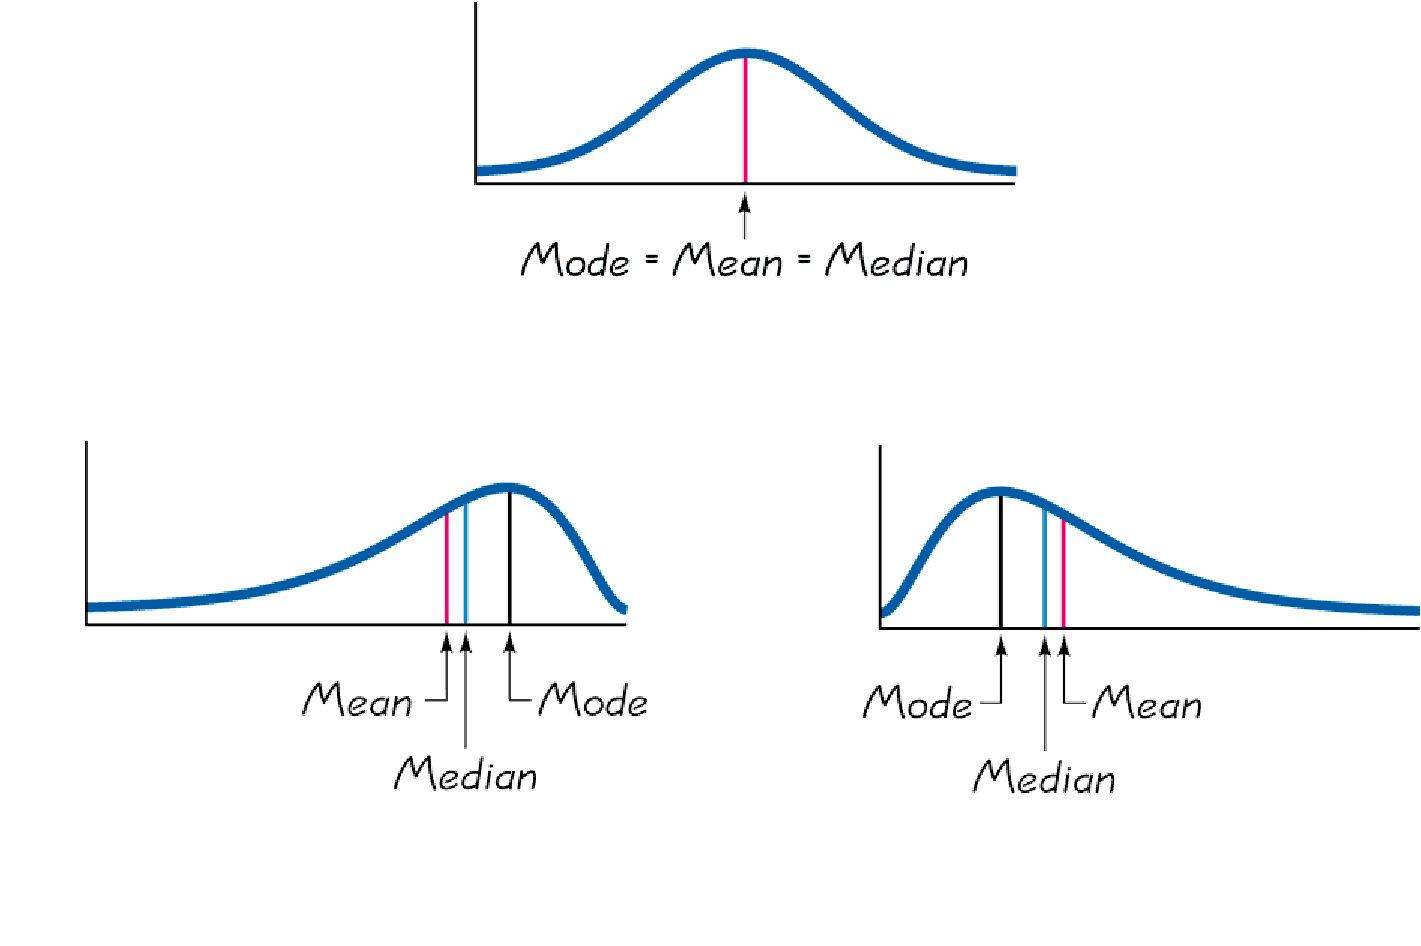
\includegraphics[width=\textwidth]{../img/medidas-crop}
  \end{figure}
\end{frame}

\begin{frame}{Média, Mediana, e Moda}
  \textbf{Exemplo}: Os dados abaixo se referem ao percentual de
  cobertura de vegetação em duas áreas de uma floresta.
  \begin{flushleft}
    Área A: \texttt{43 47 48 51 51 55 55 57 59}
  \end{flushleft}
  \begin{flushleft}
    Área B: \texttt{20 22 45 46 53 54 56 57}
  \end{flushleft}
  \begin{itemize}
  \item[a)] Calcule a média, a mediana e a moda para a área A. Qual a
    medida de tendência central melhor representa esse conjunto de
    dados? Por quê?
    \item[b)] Calcule a média, a mediana e a moda para a área B. Qual a
      medida de tendência central melhor representa esse conjunto de
      dados? Por quê?
  \end{itemize}
\end{frame}



\section{Medidas de variação}

\begin{frame}{Introdução}
 O resumo de um conjunto de dados exclusivamente por uma medida de
 centro, \textbf{esconde} toda a informação sobre a variabilidade do
 conjunto de observações \\~\\
 Não é possível analisar um conjunto de dados apenas através de uma
 medida de tendência central \\~\\
 Por isso precisamos de medidas que resumam a \textbf{variabilidade} dos
 dados em relação à um valor central
\end{frame}

\begin{frame}{Introdução}
\begin{knitrout}\footnotesize
\definecolor{shadecolor}{rgb}{0.969, 0.969, 0.969}\color{fgcolor}

{\centering 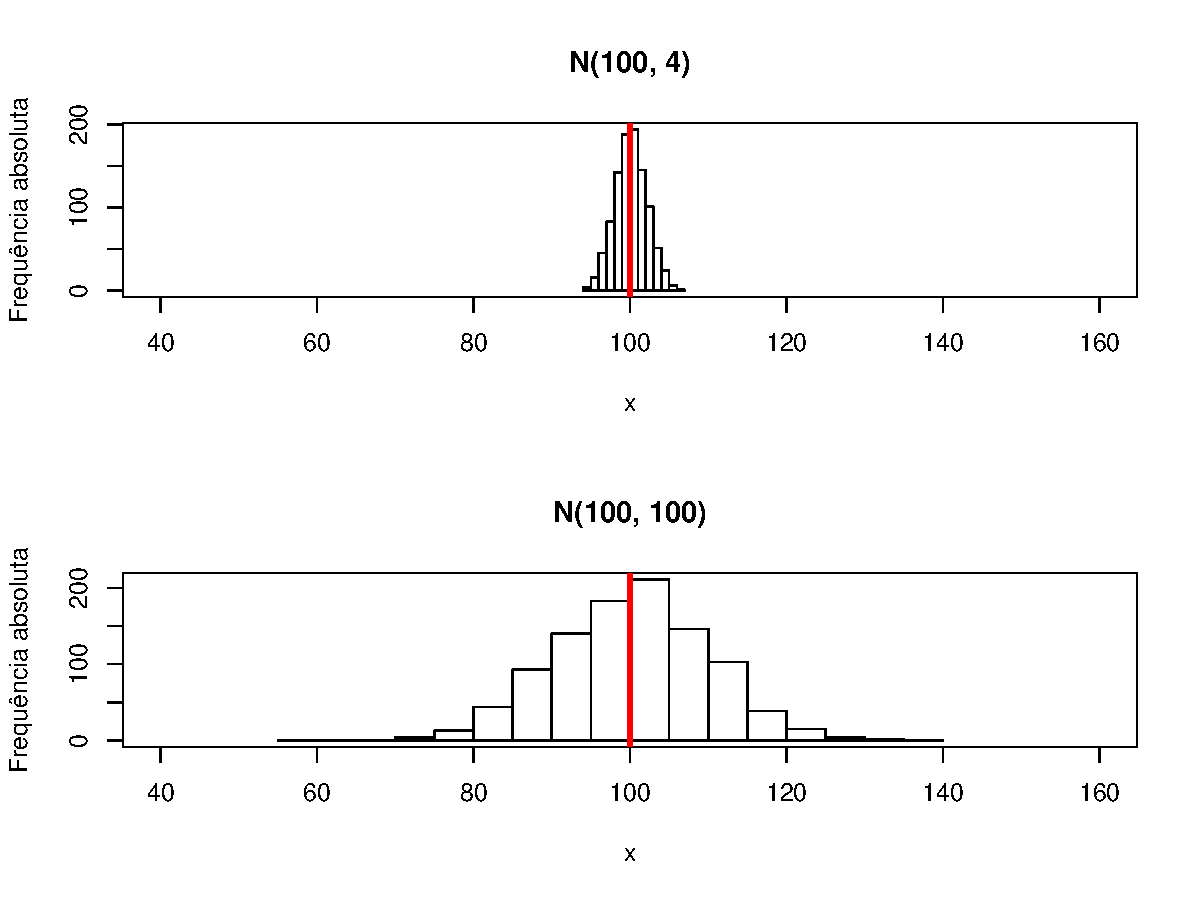
\includegraphics[width=.95\textwidth]{figure/unnamed-chunk-2-1} 

}



\end{knitrout}
\end{frame}

\begin{frame}{Introdução}
  %% Bussab, pg 37
  Cinco grupos de alunos se submeteram a um teste, obtendo as seguintes
  notas
  \begin{table}[htbp]
    \centering
    \begin{tabular}{crr}
      \hline
      \textbf{Grupo} & \textbf{Notas} & $\bar{x}$ \\ \hline
      A & 3, 4, 5, 6, 7 & 5 \\
      B & 1, 3, 5, 7, 9 & 5\\
      C & 5, 5, 5, 5, 5 & 5\\
      D & 3, 5, 5, 7 & 5\\
      E & 3, 5, 5, 6, 6 & 5\\
      \hline
    \end{tabular}
  \end{table}
  O que a média diz a respeito das notas quando comparamos os grupos?
\end{frame}

\begin{frame}{Medidas de variação}
  \begin{block}{Definição}
    São medidas estatísticas que caracterizam o quanto um conjunto de
    dados está disperso em torno de sua tendência central
  \end{block}
  \vspace{1em}
  Ferramentas para \textbf{resumo} e \textbf{análise} de dados\\~\\
  \begin{itemize}
  \item Amplitude
  \item Desvio-médio
  \item Variância
  \item Desvio-padrão
  \item Coeficiente de Variação
  \end{itemize}
\end{frame}

\subsection{Amplitude}

\begin{frame}{Amplitude}
  A \textbf{amplitude} de um conjunto de dados é a diferença entre o
  maior e o menor valor.
  \begin{equation*}
    \text{AMP} = \max - \min
  \end{equation*}
  \vspace{1em}

  Como a amplitude usa \textbf{apenas} os valores máximo e mínimo, é
  muito \textbf{sensível} a valores extremos \\~\\
\end{frame}

\begin{frame}{Amplitude}
  Calcule a média e a amplitude do número de acertos em uma prova com 50
  questões
  \begin{center}
    \texttt{31 27 42 35 47 28 7 45 15 20}
  \end{center}
  \vspace{1em}
  Calcule a média e a amplitude para a idade de um grupo de pessoas
  \begin{center}
    \texttt{4 3 4 3 4 3 21}
  \end{center}
\end{frame}

\begin{frame}{Medidas de variação}
  Para melhorar a medida de variabilidade, devemos considerar
  \textbf{todos os dados disponíveis} \\~\\
  A melhor forma de se fazer isso é considerar o \textbf{desvio} de cada
  valor em relação à média \\~\\
  Como queremos um \textbf{resumo} da variabilidade, devemos fazer a
  \textbf{soma} dos desvios \\~\\
  Considere as notas do grupo A do exemplo acima ($\bar{x} = 5$)
    \begin{table}[htbp]
    \centering
    \begin{tabular}{cc}
      \hline
      \textbf{Grupo A} & $x_i - \bar{x}$ \\ \hline
      3 & -2 \\
      4 & -1\\
      5 & 0\\
      6 & 1\\
      7 & 2\\
      \hline
      Soma & 0 \\
      \hline
    \end{tabular}
  \end{table}
\end{frame}

\begin{frame}{Medidas de variação}
  Como a soma dos desvios é \textbf{sempre} zero, temos duas alternativas
  \begin{itemize}
  \item Considerar o total dos desvios absolutos (em módulo)
    \begin{equation*}
      \sum_{i=1}^{n} |x_i - \bar{x}|
    \end{equation*}
  \item Considerar o total dos quadrados dos desvios
        \begin{equation*}
      \sum_{i=1}^{n} (x_i - \bar{x})^2
    \end{equation*}
  \end{itemize}
  O uso destes totais pode causar dificuldades quando comparamos
  conjuntos de dados de tamanhos diferentes.
  Desse modo é mais conveniente exprimir estas medidas como
  \textbf{médias} (dividindo as somas por $n$). Assim teremos:
  \begin{itemize}
  \item Desvio médio
  \item Variância
  \end{itemize}
\end{frame}

\subsection{Desvio médio}

\begin{frame}{Desvio médio}
  O \textbf{desvio médio} é definido como a média aritmética dos desvios
  em módulo (valor absoluto)
  \begin{equation*}
    \text{DM} = \frac{1}{n} \sum_{i=1}^{n} |x_i - \bar{x}|
  \end{equation*}
    No exemplo anterior
    \begin{table}[htbp]
    \centering
    \begin{tabular}{ccc}
      \hline
      \textbf{Grupo A} & $x_i - \bar{x}$ & $|x_i - \bar{x}|$ \\ \hline
      3 & -2 & 2 \\
      4 & -1 & 1\\
      5 & 0 & 0\\
      6 & 1 & 1\\
      7 & 2 & 2\\
      \hline
      Soma & 0 & 6\\
      \hline
    \end{tabular}
  \end{table}
  $\text{DM} = \frac{6}{5} = 1,2$
\end{frame}

\begin{frame}{Desvio médio}
  Mas, o desvio médio é baseado em uma operação \textbf{não algébrica}
  (módulo), o que cria dificuldades em análises posteriores \\~\\
  Além disso, é uma medida \textbf{viesada} \\~\\
  Uma alternativa melhor é a \textbf{soma dos quadrados dos desvios}
\end{frame}

\subsection{Variância}

\begin{frame}{Variância}
  A \textbf{variância} é definida como a \textit{média aritmética} da
  soma dos quadrados dos desvios.\\~\\
  \textbf{Variância amostral}
  \begin{equation*}
    s^2 = \frac{1}{n} \sum_{i=1}^{n} (x_i - \bar{x})^2
  \end{equation*}
  Uma fórmula alternativa da variância pode ser obtida desenvolvendo-se
  o quadrado no numerador da expressão anterior \\~\\
  \begin{equation*}
    s^2 = \frac{1}{n} \left[ \sum_{i=1}^{n} x_{i}^{2} -
    \frac{(\sum_{i=1}^{n} x_i)^2}{n} \right]
  \end{equation*}
\end{frame}

\begin{frame}{Variância}
  No exemplo anterior
    \begin{table}[htbp]
    \centering
    \begin{tabular}{cccc}
      \hline
      \textbf{Grupo A} & $x_i - \bar{x}$ & $|x_i - \bar{x}|$ & $(x_i -
      \bar{x})^2$ \\ \hline
      3 & -2 & 2 & 4 \\
      4 & -1 & 1 & 1\\
      5 & 0 & 0 & 0\\
      6 & 1 & 1 & 1\\
      7 & 2 & 2 & 4\\
      \hline
      Soma & 0 & 6 & 10\\
      \hline
    \end{tabular}
  \end{table}
  $s^2 = \frac{10}{5} = 2$ \\~\\
\end{frame}

\begin{frame}{Variância}
  Assim como no caso da média, se tivermos $n$ observações da variável
  $X$, das quais $f_1$ são iguais a $x_1$, $f_2$ são iguais a $x_2$,
  \ldots, $f_k$ são iguais a $x_k$, então a variância pode ser definida
  por:
  \begin{equation*}
    s^2 = \frac{1}{n} \sum_{i=1}^{n} f_i (x_i - \bar{x})^2 =
    \sum_{i=1}^{n} fr_i (x_i - \bar{x})^2
  \end{equation*}
  Ou, pela fórmula alternativa
  \begin{eqnarray*}
    s^2 &=& \frac{1}{n} \left[ \sum_{i=1}^{n} x_{i}^{2} \cdot f_i -
    \frac{(\sum_{i=1}^{n} x_i \cdot f_i)^2}{n} \right] \\
        &=& \sum_{i=1}^{n} x_{i}^{2} \cdot fr_i -
    \frac{(\sum_{i=1}^{n} x_i \cdot fr_i)^2}{n}
  \end{eqnarray*}
\end{frame}

\begin{frame}{Variância}
  Como exemplo, considere a tabela de frequência abaixo ($\bar{x} =
  1,65$):
  \begin{table}[h]
    \centering
    \begin{tabular}{cccc}
      \hline
      \textbf{Número} & \textbf{$f_i$} & \textbf{$fr_i$} & \textbf{$x_i - \bar{x}$} \\
      \hline
      0 & 4 & 0,20 & -1,65 \\
      1 & 5 & 0,25 & -0,65 \\
      2 & 7 & 0,35 & 0,35 \\
      3 & 3 & 0,15 & 1,35 \\
      5 & 1 & 0,05 & 3,35 \\
      \hline
      \textbf{Total} & 20 & 1 & \\
      \hline
    \end{tabular}
  \end{table}
  A variância pode ser calculada por:
  \begin{eqnarray*}
    s^2 &=& \frac{1}{20} \cdot [4 \cdot (-1,65)^2 + 5 \cdot (-0,65)^2 + \cdots + 1 \cdot (3,35)^2]\\
            &=& \frac{1}{20} \cdot (30,55)\\
            &=& 1,528
  \end{eqnarray*}
\end{frame}



\begin{frame}{Variância}
  Considere a seguinte tabela de distribuição de frequência ($\bar{x} = 11,22$):
    \begin{table}[h]
    \centering
    \begin{tabular}{lccc}
      \hline
      \textbf{Classe} & \textbf{$f_i$} & \textbf{$fr_i$} & \textbf{$x_i - \bar{x}$} \\
      \hline
      $[4,8)$ & 10 & 0,278 & -5,222 \\
      $[8,12)$ & 12 & 0,333 & -1,222 \\
      $[12,16)$ & 8 & 0,222 & 2,778 \\
      $[16,20)$ & 5 & 0,139 & 6,778 \\
      $[20,24)$ & 1 & 0,028 & 10, 778 \\
      \hline
      \textbf{Total} & 36 & 1 & \\
      \hline
    \end{tabular}
  \end{table}
  Considerando os pontos médios de cada classe, a variância pode ser calculada por
    \begin{eqnarray*}
    \bar{x} &=& \frac{1}{36} \cdot [6 \cdot (-5,222)^2 + 10 \cdot (-1,222)^2 + \cdots + 22 \cdot (10,778)^2]\\
            &=& \frac{1}{36} \cdot (698,22)\\
            &=& 19,395
  \end{eqnarray*}
\end{frame}



\begin{frame}{Variância}
  A variância amostral $s^2$ é considerada um estimador \textbf{não viesado}
  da variância populacional $\sigma^2$ \\~\\
  É utilizada em diversos métodos estatísticos e caracteriza todas as
  distribuições de probabilidade \\~\\
  No entanto, as \textsl{unidades da variância são diferentes das
    unidades dos dados originais} (são medidas ao quadrado, como notas
  ao quadrado ou cm$^2$)
\end{frame}

\subsection{Desvio-padrão}

\begin{frame}{Desvio-padrão}
  O \textbf{desvio-padrão} é a raiz quadrada da variância\\~\\
  \textbf{Desvio-padrão amostral}
  \begin{equation*}
    s = \sqrt{s^2}
  \end{equation*}
  Sendo que $s^2$ é calculada de qualquer uma das formas anteriores.
\end{frame}

\begin{frame}{Desvio-padrão}
  \textbf{Propriedades do desvio-padrão} \vspace{1em}
  \begin{itemize}
  \item É uma medida de variação de todos os dados em relação à
    \textbf{média}
  \item É sempre positivo ou nulo
    \begin{itemize}
    \item Valores mais distantes da média tem desvio-padrão maior
    \item Valores mais próximos da média tem desvio-padrão menor
    \end{itemize}
  \item A unidade do desvio-padrão é a mesma dos dados originais (por
    exemplo notas ou cm)
  \item A inclusão de valores \textbf{extremos} pode afetar
    drasticamente o valor do desvio-padrão
  \end{itemize}
\end{frame}

%% \begin{frame}{Desvio-padrão}
%%   Calcule o desvio-padrão para as notas de provas de duas turmas (em
%%   ambas $\mu=5$)
%%   \begin{center}
%%     Turma A: \texttt{0 2 4 5 5 6 8 10} \\ \vspace{1em}
%%     Turma B: \texttt{4 4,5 5 5 5 5 5,5 6}
%%   \end{center}
%%   Podemos comparar estas duas medidas? O que podemos concluir?
%% \end{frame}



\begin{frame}{Desvio-padrão}
  \textbf{Exemplo}: Os dados abaixo se referem ao percentual de
  cobertura de vegetação em duas áreas de uma floresta.
  \begin{flushleft}
    Área A: \texttt{43 47 48 51 51 55 55 57 59}
  \end{flushleft}
  \begin{flushleft}
    Área B: \texttt{20 22 45 46 53 54 56 57}
  \end{flushleft}
  \begin{itemize}
  \item[a)] Calcule o desvio-padrão para as duas áreas.
  \item[b)] Podemos comparar essas duas medidas? O que podemos concluir?
  \end{itemize}
\end{frame}



\subsection{Coeficiente de Variação}

\begin{frame}{Coeficiente de Variação}
  O \textbf{Coeficiente de Variação} (CV) mede a dispersão dos dados em
  relação à média (medido em \%)\\ \vspace{1em}
\textbf{Coeficiente de variação amostral}
  \begin{equation*}
    \text{CV} = \frac{s}{\bar{x}} \cdot 100\%
  \end{equation*}
  É utilizado para se comparar a variação de um ou mais conjuntos de
  dados
\end{frame}

\begin{frame}{Coeficiente de Variação}
  Qual o Coeficiente de Variação para as duas áreas do exemplo anterior:
  \begin{flushleft}
    Área A: \texttt{43 47 48 51 51 55 55 57 59}
  \end{flushleft}
  \begin{flushleft}
    Área B: \texttt{20 22 45 46 53 54 56 57}
  \end{flushleft}
  O que podemos concluir?
\end{frame}

\begin{frame}{Coeficiente de Variação}
  O Coeficiente de Variação é muito útil também para se comparar dados
  medidos em escalas diferentes. Por exemplo
  \begin{table}[h]
    \centering
    \begin{tabular}{ccc}
      \hline
            & Média & Desvio-padrão \\
            \hline
            Altura & 174 cm & 7 cm \\
            Peso & 78 kg & 12 kg \\
            \hline
    \end{tabular}
  \end{table}
  Sópodemos comparar o desvio-padrão com unidades diferentes através do CV
  \begin{equation*}
    \text{CV}_A = \frac{7}{174} \cdot 100\% =  4\%
    \quad \quad \text{CV}_P = \frac{12}{78} \cdot 100\% = 15,4\%
  \end{equation*}
\end{frame}

\subsection{Exercícios}

\begin{frame}{Exerícios}
  Considere a tabela de frequência abaixo:
  \begin{table}[h]
    \centering
    \begin{tabular}{cc}
      \hline
      Classe & $f_i$ \\
      \hline
      $1,0 \vdash 2,5$ & 3 \\
      $2,5 \vdash 4,0$ & 5 \\
      $4,0 \vdash 5,5$ & 3 \\
      $5,5 \vdash 7,0$ & 7 \\
      $7,0 \vdash 8,5$ & 9 \\
      $8,5 \vdash 10,0$ & 13 \\
      \hline
    \end{tabular}
  \end{table}
  Calcule a média, a variância, o desvio-padrão, e o CV para este
  conjunto de dados.
\end{frame}

\section[Medidas de posição]{Medidas de posição relativa}

\subsection{Percentis}

\begin{frame}{Percentis}
  \begin{block}{Definição}
    Percentis são medidas de posição, denotados por $P_1, P_2,
    \ldots, P_{99}$ que dividem os dados em 100 grupos, com cerca de 1\%
    cada grupo
  \end{block}
  Por exemplo
  \begin{itemize}
  \item O 50$^o$ percentil, $P_{50}$, tem cerca de 50\% dos valores
    abaixo dele, e 50\% de valores acima dele
    \begin{itemize}
    \item Nesse caso, $P_{50}$ = Mediana
    \end{itemize}
  \end{itemize}
\end{frame}

\begin{frame}[fragile]{Percentis}
  Para determinar um percentil:
  \begin{itemize}
  \item Encontre a posição
    \begin{equation*}
      \text{Pos} P_i = \frac{i(n+1)}{100}, \quad i=1,\ldots,99
    \end{equation*}
  \item Se o valor for fracionário calcule o valor intermediário
  \end{itemize}
  Calcule o $P_{30}$ e o $P_{65}$ para os dados abaixo
  \begin{center}
    \texttt{15 21 28 25 30 11 17 12 25 20 16 23 12 10}
  \end{center}

\end{frame}

\subsection{Quartis}

\begin{frame}{Quartis}
  \begin{block}{Definição}
    Quartis são medidas de posição, denotadas por $Q_1, Q_2, Q_3$
    que dividem um conjunto de dados em 4 grupos, com cerca de 25\% dos
    valores em cada grupo
  \end{block}
  \textbf{$Q_1$ (Primeiro quartil)}: Separa os 25\% inferiores dos 75\%
  superiores dos valores ordenados\\~\\
  \textbf{$Q_2$ (Segundo quartil)}: O mesmo que a mediana. Separa os
  50\% valores ordenados inferiores dos 50\% superiores\\~\\
  \textbf{$Q_3$ (terceiro quartil)}: Separa os 75\% valores ordenados
  inferiores dos 25\% superiores\\~\\
\end{frame}

\begin{frame}{Quartis}
  Para determinar um quartil:
  \begin{itemize}
  \item Encontre a posição
    \begin{equation*}
      \text{Pos} Q_i = \frac{i(n+1)}{4}, \quad i=1,\ldots,3
    \end{equation*}
  \item Se o valor for fracionário calcule o valor intermediário
  \end{itemize}
  Calcule os quartis para os dados abaixo
  \begin{center}
    \texttt{15 21 28 25 30 11 17 12 25 20 16 23 12 10}
  \end{center}

\end{frame}

\begin{frame}{Quartis}
  \textbf{Gráfico de caixa ou resumo dos cinco números}\\~\\
  \begin{block}{Resumo dos 5 números}
    O resumo dos cinco números consiste no valor mínimo, primeiro
    quartil, segundo quartil (mediana), terceiro quartil, e no valor
    máximo
  \end{block}
  \begin{block}{Gráfico de caixa}
    O gráfico de caixa, ou \textsl{boxplot}, é uma representação gráfica
    do resumo dos cinco números
  \end{block}
\end{frame}

\begin{frame}{Quartis}
  Para os valores
  \begin{center}
    \texttt{15 21 28 25 30 11 17 12 25 20 16 23 12 10}
  \end{center}
  o \textbf{gráfico de caixa} correspondente é
\begin{knitrout}\footnotesize
\definecolor{shadecolor}{rgb}{0.969, 0.969, 0.969}\color{fgcolor}

{\centering 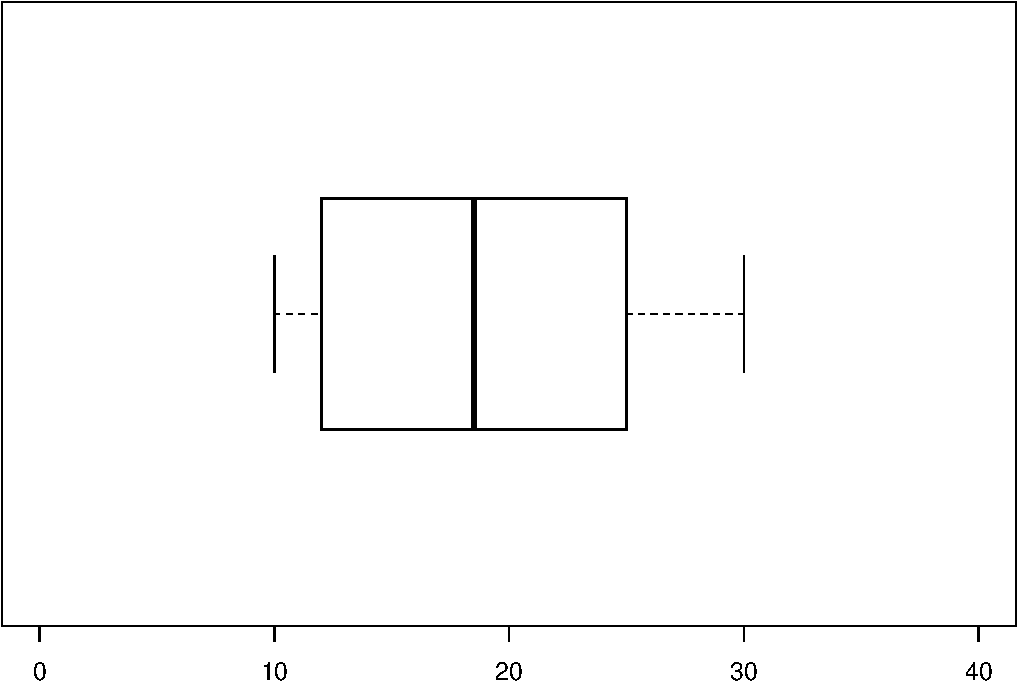
\includegraphics[width=.8\textwidth]{figure/unnamed-chunk-9-1} 

}



\end{knitrout}
\end{frame}


\begin{frame}{Quartis}
  \textbf{Gráfico de caixa ou resumo dos cinco números}\\~\\
\begin{knitrout}\footnotesize
\definecolor{shadecolor}{rgb}{0.969, 0.969, 0.969}\color{fgcolor}

{\centering 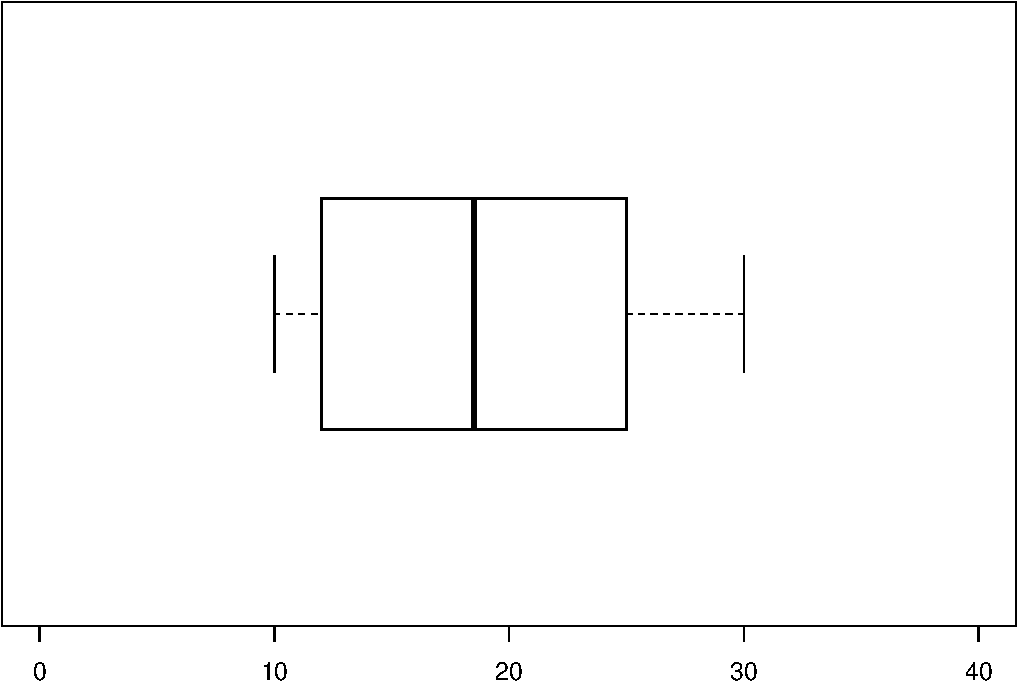
\includegraphics[width=.9\textwidth]{figure/unnamed-chunk-10-1} 

}



\end{knitrout}
\end{frame}

\begin{frame}{Quartis}
  Exemplo: o tempo de espera, em minutos, para o atendimento em uma
  central telefônica, para homens e mulheres, foi registrado como abaixo
  \begin{center}
    Homens: \texttt{5 2 7 9 3 4 3 1 3 8}\\
    Mulheres: \texttt{3 5 7 4 5 6 7 6 5 4}
  \end{center}
  \begin{itemize}
  \item Monte o resumo dos cinco números e o gráfico de caixa para
    homens e mulheres juntos
  \item Monte o resumo dos cinco números e o gráfico de caixa para
    homens e mulheres separados
  \end{itemize}

\end{frame}

\begin{frame}{Quartis}
\begin{knitrout}\footnotesize
\definecolor{shadecolor}{rgb}{0.969, 0.969, 0.969}\color{fgcolor}

{\centering 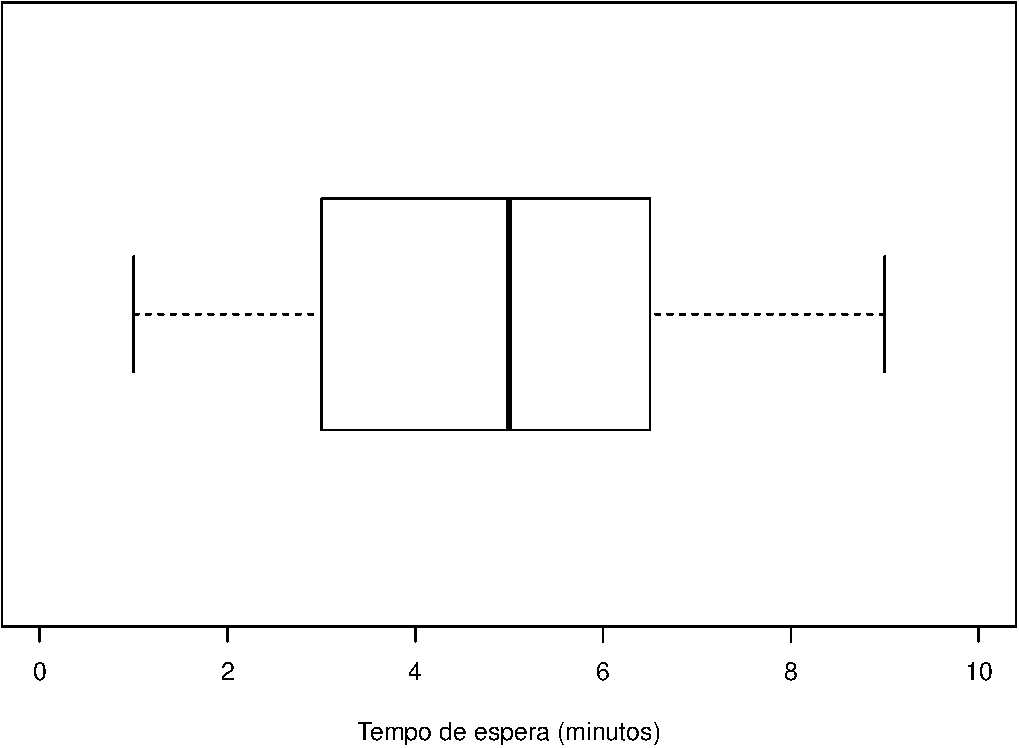
\includegraphics[width=.8\textwidth]{figure/quartis1-1} 

}



\end{knitrout}
\end{frame}

\begin{frame}{Quartis}
\begin{knitrout}\footnotesize
\definecolor{shadecolor}{rgb}{0.969, 0.969, 0.969}\color{fgcolor}

{\centering 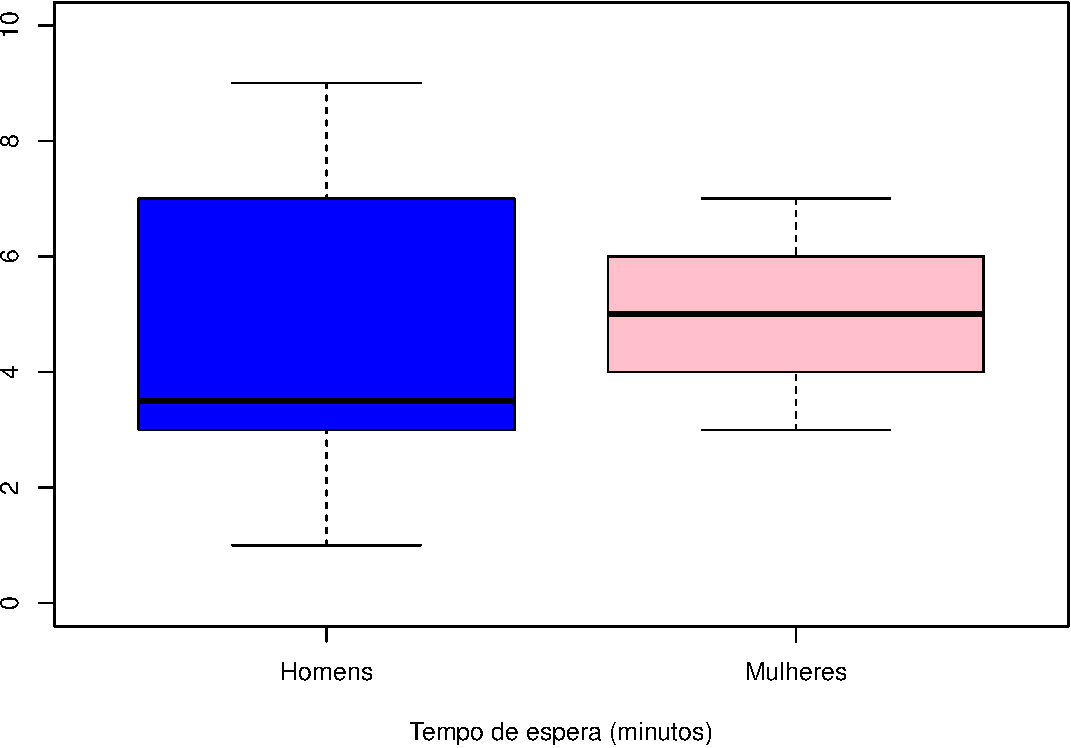
\includegraphics[width=.8\textwidth]{figure/quartis2-1} 

}



\end{knitrout}
\end{frame}

\section{Exercícios}

\begin{frame}[fragile]{Exercícios}
  Exercícios 2--7, 9--15 do capítulo 3 do livro (pgs. 94--96).
  \vspace{1em}
  \begin{itemize}
  \item[] Pinto, SS; Silva, CS. \textbf{Estatística, Vol I}. Rio Grande:
    Editora da FURG, 2010. [Cap. 3]
  \end{itemize}
\end{frame}

\begin{frame}{Referências}
  \begin{itemize}
  \item Magalhães, MN; Lima, ACP. \textbf{Noções de Probabilidade e
    Estatística}. São Paulo: EDUSP, 2008. [Cap. 1]
  \item Bussab, WO; Morettin, PA. \textbf{Estatística básica}. São
    Paulo: Saraiva, 2006. 526 p. [Cap. 3]
  \end{itemize}
\end{frame}




\end{document}
